\section{Introduction}
\ref{sec:intro}

Stepper is a programming tool that can display all immediate states of a program, which is useful for debugging and educating. It simplifies expression step by step so that people can track the evaluation procedure to find error easily. \Hazel, a programming language environment developed by [citation Cyrus Omar], assigns semantic meaning to incomplete program. It contains a special variable called hole indicating the place that is empty and needs to fill. In this paper, we want to develop an interactive stepper for \Hazel. Take the following programs as examples:

\begin{figure}[htbp]
  \centering
  \begin{subfigure}[b]{0.4\textwidth}
      \centering
      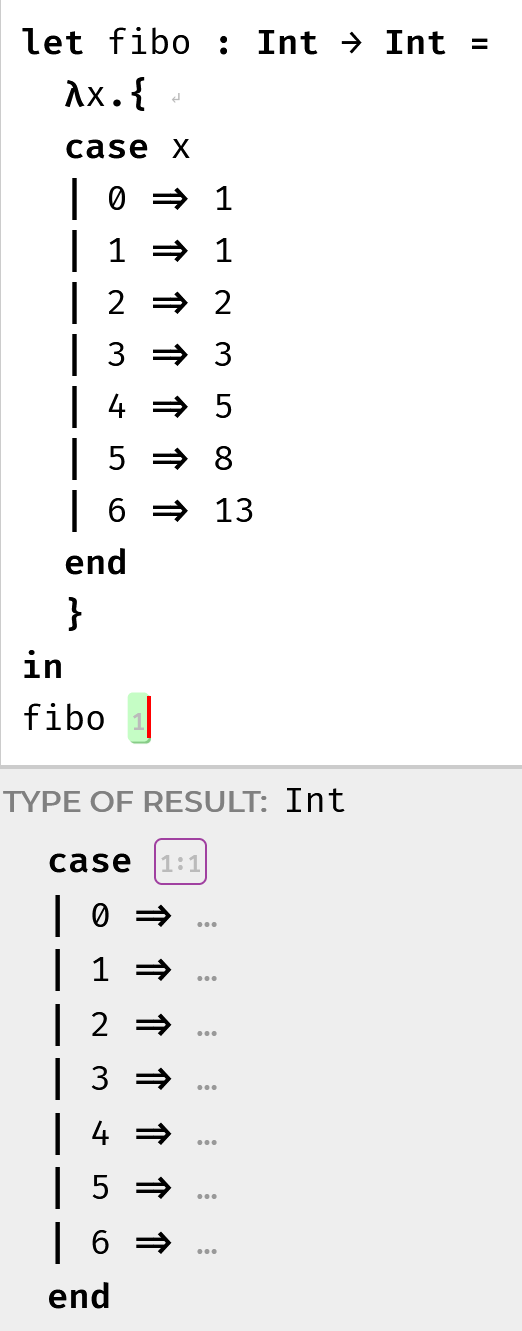
\includegraphics[width=0.5\textwidth]{img/pause_example.png}
      \caption{Example of paused environment}
      \label{fig:pause}
  \end{subfigure}
  \hfill
  \begin{subfigure}[b]{0.4\textwidth}
      \centering
      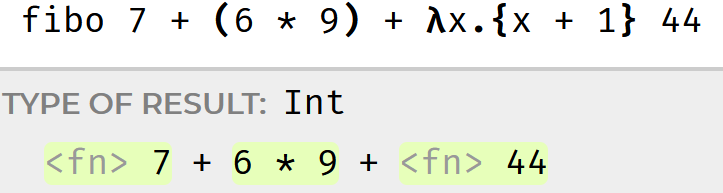
\includegraphics[width=\textwidth]{img/interactive.png}
      \caption{Example of multiple environment}
      \label{fig:multiple}
  \end{subfigure}
    \caption{Two programs in \Hazel}
    \label{fig:intro_example}
\end{figure}

% Findler et al.[citation] developed a stepper for DrScheme in their programming environment. Cong and Asai [citation] used the contextual dynamics to build a stepper, which takes subexpression out and plug in after evaluation. In this paper, we will use the similar strategy to develop the stepper. 

Figure \ref{fig:pause} is an example of expression with a hole. The evaluation result is a case expression with empty parameter. However, the origin expression is already simple enough and it is unnecessary to expand like that especially when there are many cases in the function. Therefore, we want to develop a stepper that can detect this situation so that it will pause until user requires it to step further.

Figure \ref{fig:multiple} shows an expression with three parts. The left part is heavy since it takes many steps to evaluate. However, user might just want to debug the right lambda part. According to the regular dynamics, there should contain only one way to step for any non-final programs. So, user has to click many times to reduce the left one in order to debug the right one. Our solution is to provide options for user to choose where to step. In the Figure \ref{fig:multiple}, the green boxes contain subexpressions that can be evaluated. So, stepper allows the multiple evaluation contexts so that user can choose the subexpression they need.

Our interactive stepper develops pausing environment and a simple algorithm to decompose multiple evaluation contexts. Furthermore, it also has a webview so that user can click boxes to step expressions.

\parahead{Contributions} The contributions of this paper are: (1) a pausing environment in section ~\ref{sec:pause}; (2) an algorithm to decompose multiple evaluation contexts in section ~\ref{sec:condy}.